\chapter{Heritability of Schizophrenia}

\section{Introduction}
Apply Heritability estimation to the schizophrenia data.
The genetic correlation and partitioning of heritability
No one worked on linking schizophrenia with brain development directly?
% talk about the current research on schizophrenia?
% the overall heritablity estimation
% The genetic correlation done by the LDSC. 
% The theory of brain development 
% How the co-expression network works
% Drug response?
\section{Heritability Estimation}
This will be a very simple section, focused on how to perform the heritability estimation on \acrfull{scz}.
Should also tokenize the heritability into subcategories (e.g. immune, neuron, etc)
%Should not put too much weight into it, otherwise it will be a direct copy of LDSC. Won't really add much power. 


\subsection{Methodology}
\subsection{Result}
\section{Brain development and Schizophrenia}
\sectionmark{Brain development}
Here we will perform the WGCNA and brain development network.
Seeing how the whether if any brain development network were enriched with SNPs that explain the variance of phenotype
%Instead, we should put most focus here as no one has done it before
%Also descript brainspan here
\subsection{Methodology}
\subsubsection{Sample Quality Controls}
We obtain the developmental transcriptome data from BrainSpan (\url{http://www.brainspan.org/}). 
A total of 56 samples with different age were provided by BrainSpan with an average of 2.2 samples per age.

Studies suggested Hippocampus\citep{Velakoulis2006,Nugent2007}, Amygdala and Striatum\citep{Simpson2010} are brain regions involved in the etiology of schizophrenia. 
Therefore, we focus on building the gene co-expression network of hippocampus, amygdala and striatum in this study
It is worth noting that the Pre-frontal Cortex is also important for schizophrenia. 
However, as there isn't a well defined pre-frontal cortex samples from BrainSpan, we did not include the pre-frontal cortex in the current study.
RNA Sequencing data of the brain regions were obtained from BrainSpan and undergo a series of quality control before the construction of the network. 

For each sample age, when there are more than one samples, we select the sample with a dissection score $\ge3$ and an \gls{rin} $\ge7$. 
As some developmental stage only got 1 sample passing the quality check, we limit each developmental stage to have a maximum of 1 sample such that the final network will not be driven by a particular developmental stage. 
If multiple samples passed through the quality check threshold, we will prefer sample with higher dissection score. 
Shall multiple samples have the same dissection score, we will select the one with the highest \gls{rin}. 
And if the samples have the same dissection score and \gls{rin} value, we will randomly select one for the network construction.

After performing the quality control, a total of 16, 18 and 15 samples were selected for hippocampus, amygdala and striatum respectively.
The sample age ranged from \gls{gd}8 to 23 years old representing the fetal developmental stage till the age of onset of schizophrenia.

\subsubsection{Normalization of data}
The RNA Sequencing data were represented as \gls{rpkm} values. 
Genes with a low \gls{rpkm} can usually be a result from technical or biological noise\citep{Hart2013}.
To reduce noise in the final model, genes with a mean \gls{rpkm} $< 1$ in all samples were discarded. 
The \gls{rpkm} were then log transformed as instructed by the manual of \gls{wgcna}\citep{Langfelder2008}.

As there are insufficient samples for the construction of gene co-expression network for individual sample age, we try to construct networks with genes co-expressed through all sample stage. 
This is achieved by taking the standardized log$_2$ \gls{rpkm} across sample age such that all genes has a mean of 0 and standard deviation of 1.

At the end, there were 17,168 genes, 17,038 genes and 17,166 genes passing through the quality threshold and were used for the construction of co-expression network in hippocampus, amygdala and striatum respectively. 

\subsubsection{Network Construction}
\gls{wgcna} (ver 1.47) were used for the construction of gene co-expression network\citep{Langfelder2008}. 
The \emph{blockwiseModules} function, using Biweight Midcorrelation for the construction of correlation matrix and a restriction of minimum network size of 30. 
For the construction of gene co-expression networks in hippocampus, the soft-power threshold were set to 15 where it is the first threshold value which has $R^2 > 0.8$ (0.817) and the $R^2$ is saturated\citep{Zhang2005}.%(\cref{fig:softpowerThreshold})
As for striatum, the soft-power threshold were set to 20. 
Again, this is the first threshold value with $R^2 >0.8$ (0.879) and where the $R^2$ is saturated.

On the other hand, for amygdala, soft-power threshold were set to 9 which is the first threshold for $R^2$ to reach saturation. 
However, with a soft-power threshold of 9, the $R^2$ were only 0.776, which is lower than the recommended 0.8 threshold.
The reason behind this decision was that the first soft-power threshold to have $R^2 > 0.8$ is 30.
Under this threshold, the mean connectivity of the resulting networks will be around 23.6 with a median connectivity of 2.51.
Such level of connectivity will likely yield networks that are too small to useful.
If one would like to satisfy both requirement of threshold selection, a threshold $>30$ are likely required and any networks constructed will likely to be small.
As a result of that, we select threshold of 9 where networks with reasonable size can be constructed.

%\begin{figure}
%	\caption[Soft-power threshold selection]{Soft-power threshold selection. A soft-power of 13 were selected as it is the first threshold value having $R^2 > 0.8$ (0.817) and where the $R^2$ is saturated.}
%	\centering
%	\scalebox{.8}{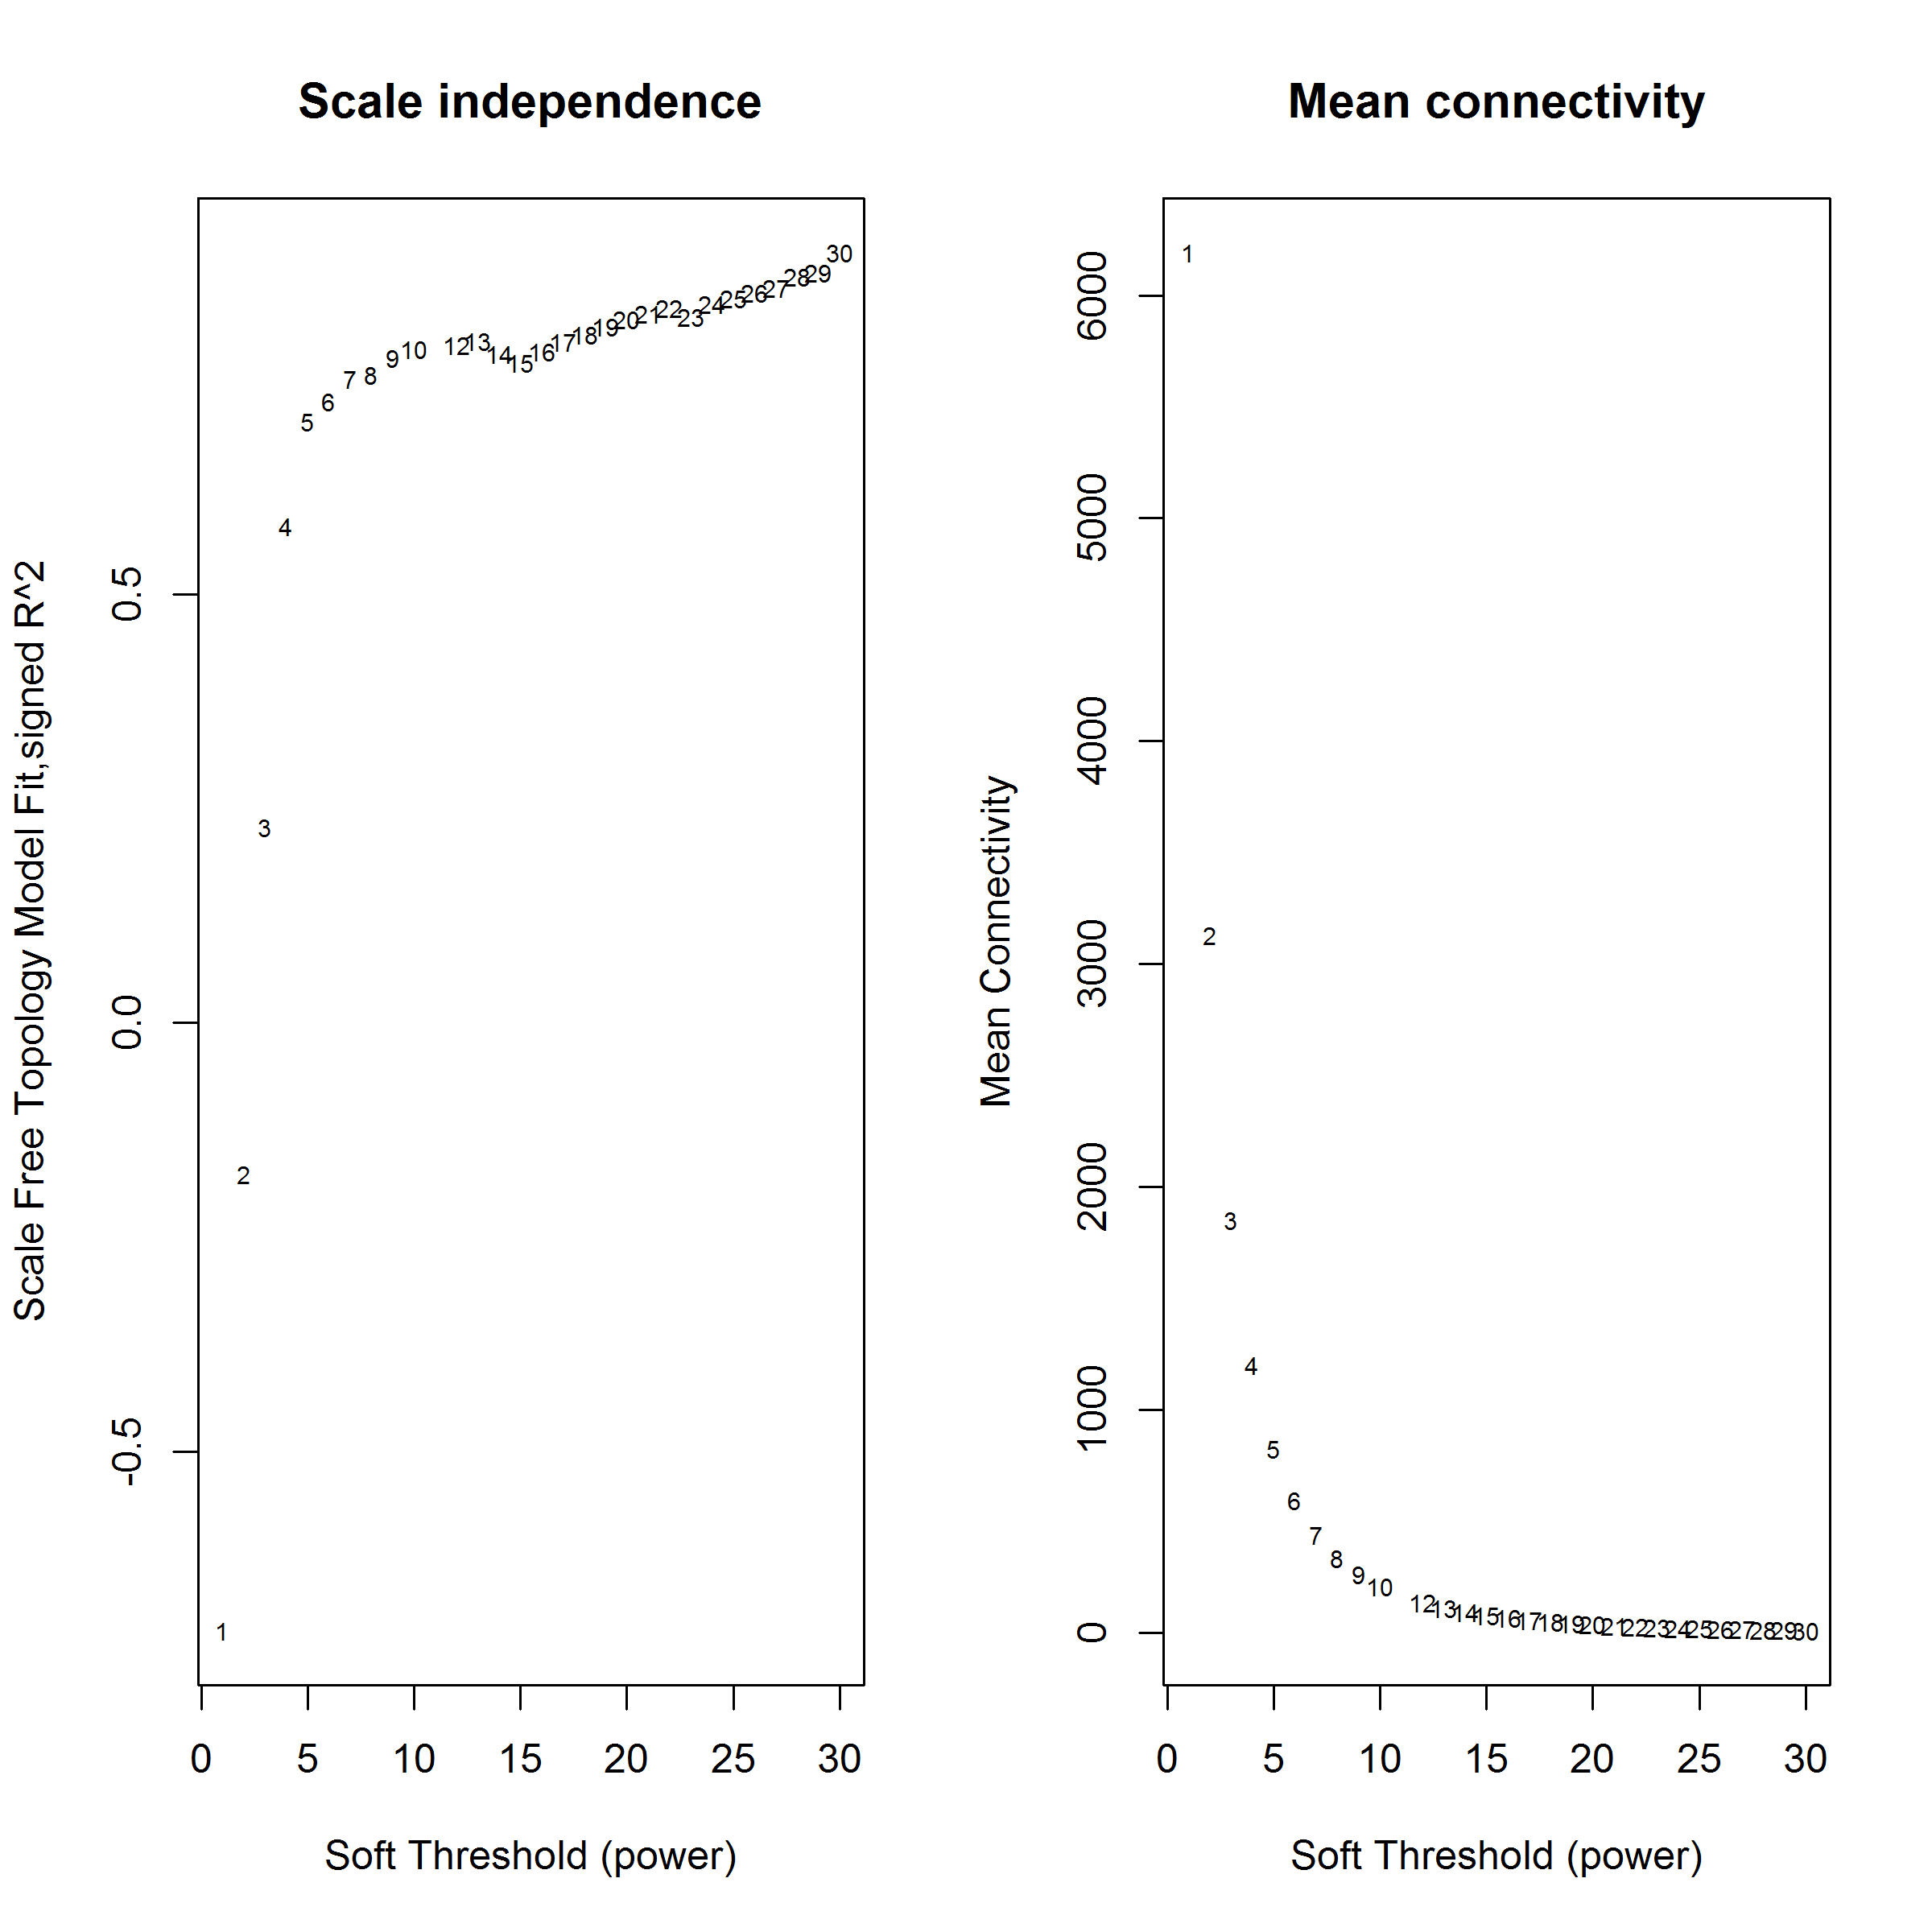
\includegraphics{figure/SoftpowerThreshold.png}}
%	\label{fig:softpowerThreshold}
%\end{figure}

\subsubsection{Expression correlation with Age}
The co-expression network constructed with the standardized gene expression value will contains genes that co-express in all sample age.
However, this does not necessary suggest the expression of these genes are correlated with the sample age.
To identify gene co-expression networks with expressions correlated with the sample age, we performed a correlation analysis between the module eigen-genes and the sample age. 
Network eigen-genes were calculated as the first \gls{pc} of expressions of the genes within individual networks using the \emph{moduleEigengenes} function from \gls{wgcna}. 
Age were represented as month from conception such that 8 post-conception week will be represented as 2; 4 months will be represented as 10 and 12 years will be represented as 154 etc. 
Finally, correlation between age and network eigen-gene expression were calculated pearson correlation.

\subsubsection{Functional Annotation}
\gls{GO} based enrichment analysis of the significant module was performed using GOrilla\citep{Eden2009}.
Genes within the networks were provide as the target gene lists and all the genes passed quality controls were used as the background gene list.
As \gls{GO} terms tends to be redundant and overlaps with each other, it will aid the interpretation of \gls{GO} results based by clustering and reducing the \gls{GO} terms based on their similarity. 
Thus, \gls{GO} enrichment results were summerized by REViGO\citep{Supek2011} and significant representative \gls{GO} terms were obtained.

\subsubsection{Associate Co-expression network with \glsentryshort{pgc} schizophrenia data}
The co-expression networks were built from normal samples and should not be representative of the brain expression pattern in schizophrenia patients.
it is however interesting to see if the co-expression networks were disrupted in schizophrenia patient.
To test whether if the gene co-expression networks contain genes that are jointly associated with schizophrenia, we first use \gls{MAGMA}\citep{DeLeeuw2015}(version v1.03) to compute the gene-base p-value from the \gls{SNP} wise p-value obtained from \gls{pgc}. 
Gene-set enrichment analysis were then performed on networks that were significantly correlated with developmental age. 
As we were only interested in whether if the genes within the networks were jointly associated with schizophrenia, we only focus on the result of the self-contained gene set analysis and ignore the result from competitive analysis.

\subsubsection{Partitioning of Heritability}

\subsection{Result}
\subsubsection{Co-Expression Network}
A total of 35 networks were constructed based on the hippocampus samples with a mean network size of 421.6.
On the other hand, 28 networks were constructed for amygdala with mean network size of 591.86.
Finally, 25 networks with mean size of 494.52 were constructed from the striatum samples.

Of the all the networks constructed, only one network from hippocampus(\cref{tab:hipModSig}) and three networks from amygdala(\cref{tab:amyModSig}) were significantly correlated with sample age after bonferroni correction threshold (p-value $<0.00143$ for hippocampus, p-value $<0.00179$ for amygdala and p-value $<0.002$ for striatum) .
\begin{table}
	\centering
	\caption[Correlation of sample age with the module eigen gene]{Correlation of sample age with the module eigen gene. 
		Module eigen-gene was defined as the first \gls{pc} of genes within the module. 
		After correcting for multiple testing, only the black module was considered as significantly correlated with the sample age.}
	\subfloat[Hippocampus]{
		\begin{tabular}{rrr}
			\toprule
			& Correlation & Pvalue \\
			\midrule
			black & 0.804653 & 0.000171 \\
			blue  & -0.61648 & 0.010981 \\
			red   & -0.60207 & 0.013595 \\
			darkred & -0.59137 & 0.015833 \\
			greenyellow & -0.56995 & 0.021168 \\
			yellow & 0.567828 & 0.021763 \\
			darkgrey & -0.55246 & 0.026474 \\
			saddlebrown & -0.52983 & 0.034783 \\
			turquoise & -0.51371 & 0.041809 \\
			purple & -0.46788 & 0.067606 \\
			darkolivegreen & -0.41272 & 0.112122 \\
			sienna3 & -0.39535 & 0.129604 \\
			darkturquoise & 0.386541 & 0.139154 \\
			darkorange & 0.384966 & 0.140912 \\
			darkmagenta & 0.375586 & 0.151688 \\
			brown & 0.366095 & 0.163144 \\
			tan   & -0.36522 & 0.164229 \\
			pink  & 0.348979 & 0.18524 \\
			magenta & -0.32559 & 0.218473 \\
			midnightblue & -0.29168 & 0.273014 \\
			lightgreen & 0.289921 & 0.276056 \\
			paleturquoise & -0.28045 & 0.29276 \\
			white & 0.27727 & 0.29849 \\
			orange & 0.19607 & 0.466754 \\
			steelblue & 0.17355 & 0.520357 \\
			skyblue & 0.145869 & 0.589857 \\
			lightyellow & -0.11665 & 0.667028 \\
			green & -0.09882 & 0.715786 \\
			violet & -0.08757 & 0.747076 \\
			lightcyan & -0.0656 & 0.809257 \\
			cyan  & -0.06441 & 0.812661 \\
			darkgreen & -0.03914 & 0.885582 \\
			salmon & 0.038727 & 0.886769 \\
			royalblue & -0.03785 & 0.889314 \\
			grey60 & 0.03119 & 0.908709 \\
			\bottomrule
			\label{tab:hipModSig}%
		\end{tabular}%
	}
	\qquad%
	\subfloat[Amygdala]{
		\begin{tabular}{rrr}
			\toprule
			& Correlation & P-value \\
			\midrule
			tan   & 0.849999 & $7.96\times 10^{-6}$ \\
			yellow & -0.757 & $2.76\times 10^{-4}$ \\
			pink  & -0.68541 & $1.69\times 10^{-3}$ \\
			greenyellow & -0.67831 & $1.97\times 10^{-3}$ \\
			red   & -0.64532 & $3.83\times 10^{-3}$ \\
			turquoise & -0.59771 & $8.80\times 10^{-3}$ \\
			lightyellow & -0.56347 & 0.0149 \\
			brown & 0.548516 & 0.0184 \\
			darkgreen & -0.46366 & 0.0526 \\
			blue  & -0.4604 & 0.0545 \\
			purple & -0.44182 & 0.0664 \\
			darkgrey & -0.39065 & 0.109 \\
			orange & -0.36966 & 0.131 \\
			white & 0.28737 & 0.248 \\
			darkred & 0.283247 & 0.255 \\
			black & 0.271383 & 0.276 \\
			salmon & -0.24203 & 0.333 \\
			skyblue & 0.207071 & 0.410 \\
			cyan  & 0.18778 & 0.456 \\
			lightgreen & 0.166495 & 0.509 \\
			grey60 & 0.15156 & 0.548 \\
			midnightblue & 0.136078 & 0.590 \\
			magenta & -0.13459 & 0.594 \\
			darkturquoise & 0.129954 & 0.607 \\
			lightcyan & 0.090241 & 0.722 \\
			darkorange & -0.05166 & 0.839 \\
			green & -0.04745 & 0.852 \\
			royalblue & 0.020456 & 0.936 \\
			\bottomrule
			\label{tab:amyModSig}%
		\end{tabular}%
	}
\end{table}

By plotting the mean expression of each network against the sample age, one can inspect how the dynamic of the network changes across different developmental stage.
Thus, mean expression of all the genes within the significant networks were calculated for all amygdala (n=33) and hippocampus (n=32) samples from BrainSpan.
The mean \gls{rpkm} values were then log$_2$ transformed and plot against the sample age where a line of bests fit was calculated using the \emph{stat\_smooth} with the loess function from R package \emph{ggplot2}(version 1.0.1). (\cref{fig:allMod}).

The expression pattern observed were intriguing where there both the ``black''(\cref{fig:blackMod}) and ``tan'' (\cref{fig:tanMod}) networks have mean gene expression level increase as development progress and reaches its peak at around late adolescence ($\approx 18-21$), concurring with the onset age of schizophrenia.
Similarly, an inverse pattern were observed with the ``yellow'' network where its mean expression was highest during fetal development and drop steadily to its lowest around late adolescence and increase again afterwards(\cref{fig:yellowMod}).

The expression pattern of the ``black'' and ``tan'' networks are of particular interest as they follow the inverted ``U'' shape trajectory of the grey matter volumn observed in previous studies\citep{Gogtay2011}, suggest that they might have a role in mediating brain development. 
\begin{figure}
	\caption[Mean Gene Expression across developmental age]{Mean Gene Experssion across developmental age.
		Mean \gls{rpkm} values of genes in the significant modules were plot with respect to the sample age.
		A loess smoothing curve was also plotted. 
		%Might want to talk somemore about it
	}
	\centering
	\subfloat[``Black'' Network from Hippocampus]{
		\scalebox{.4}{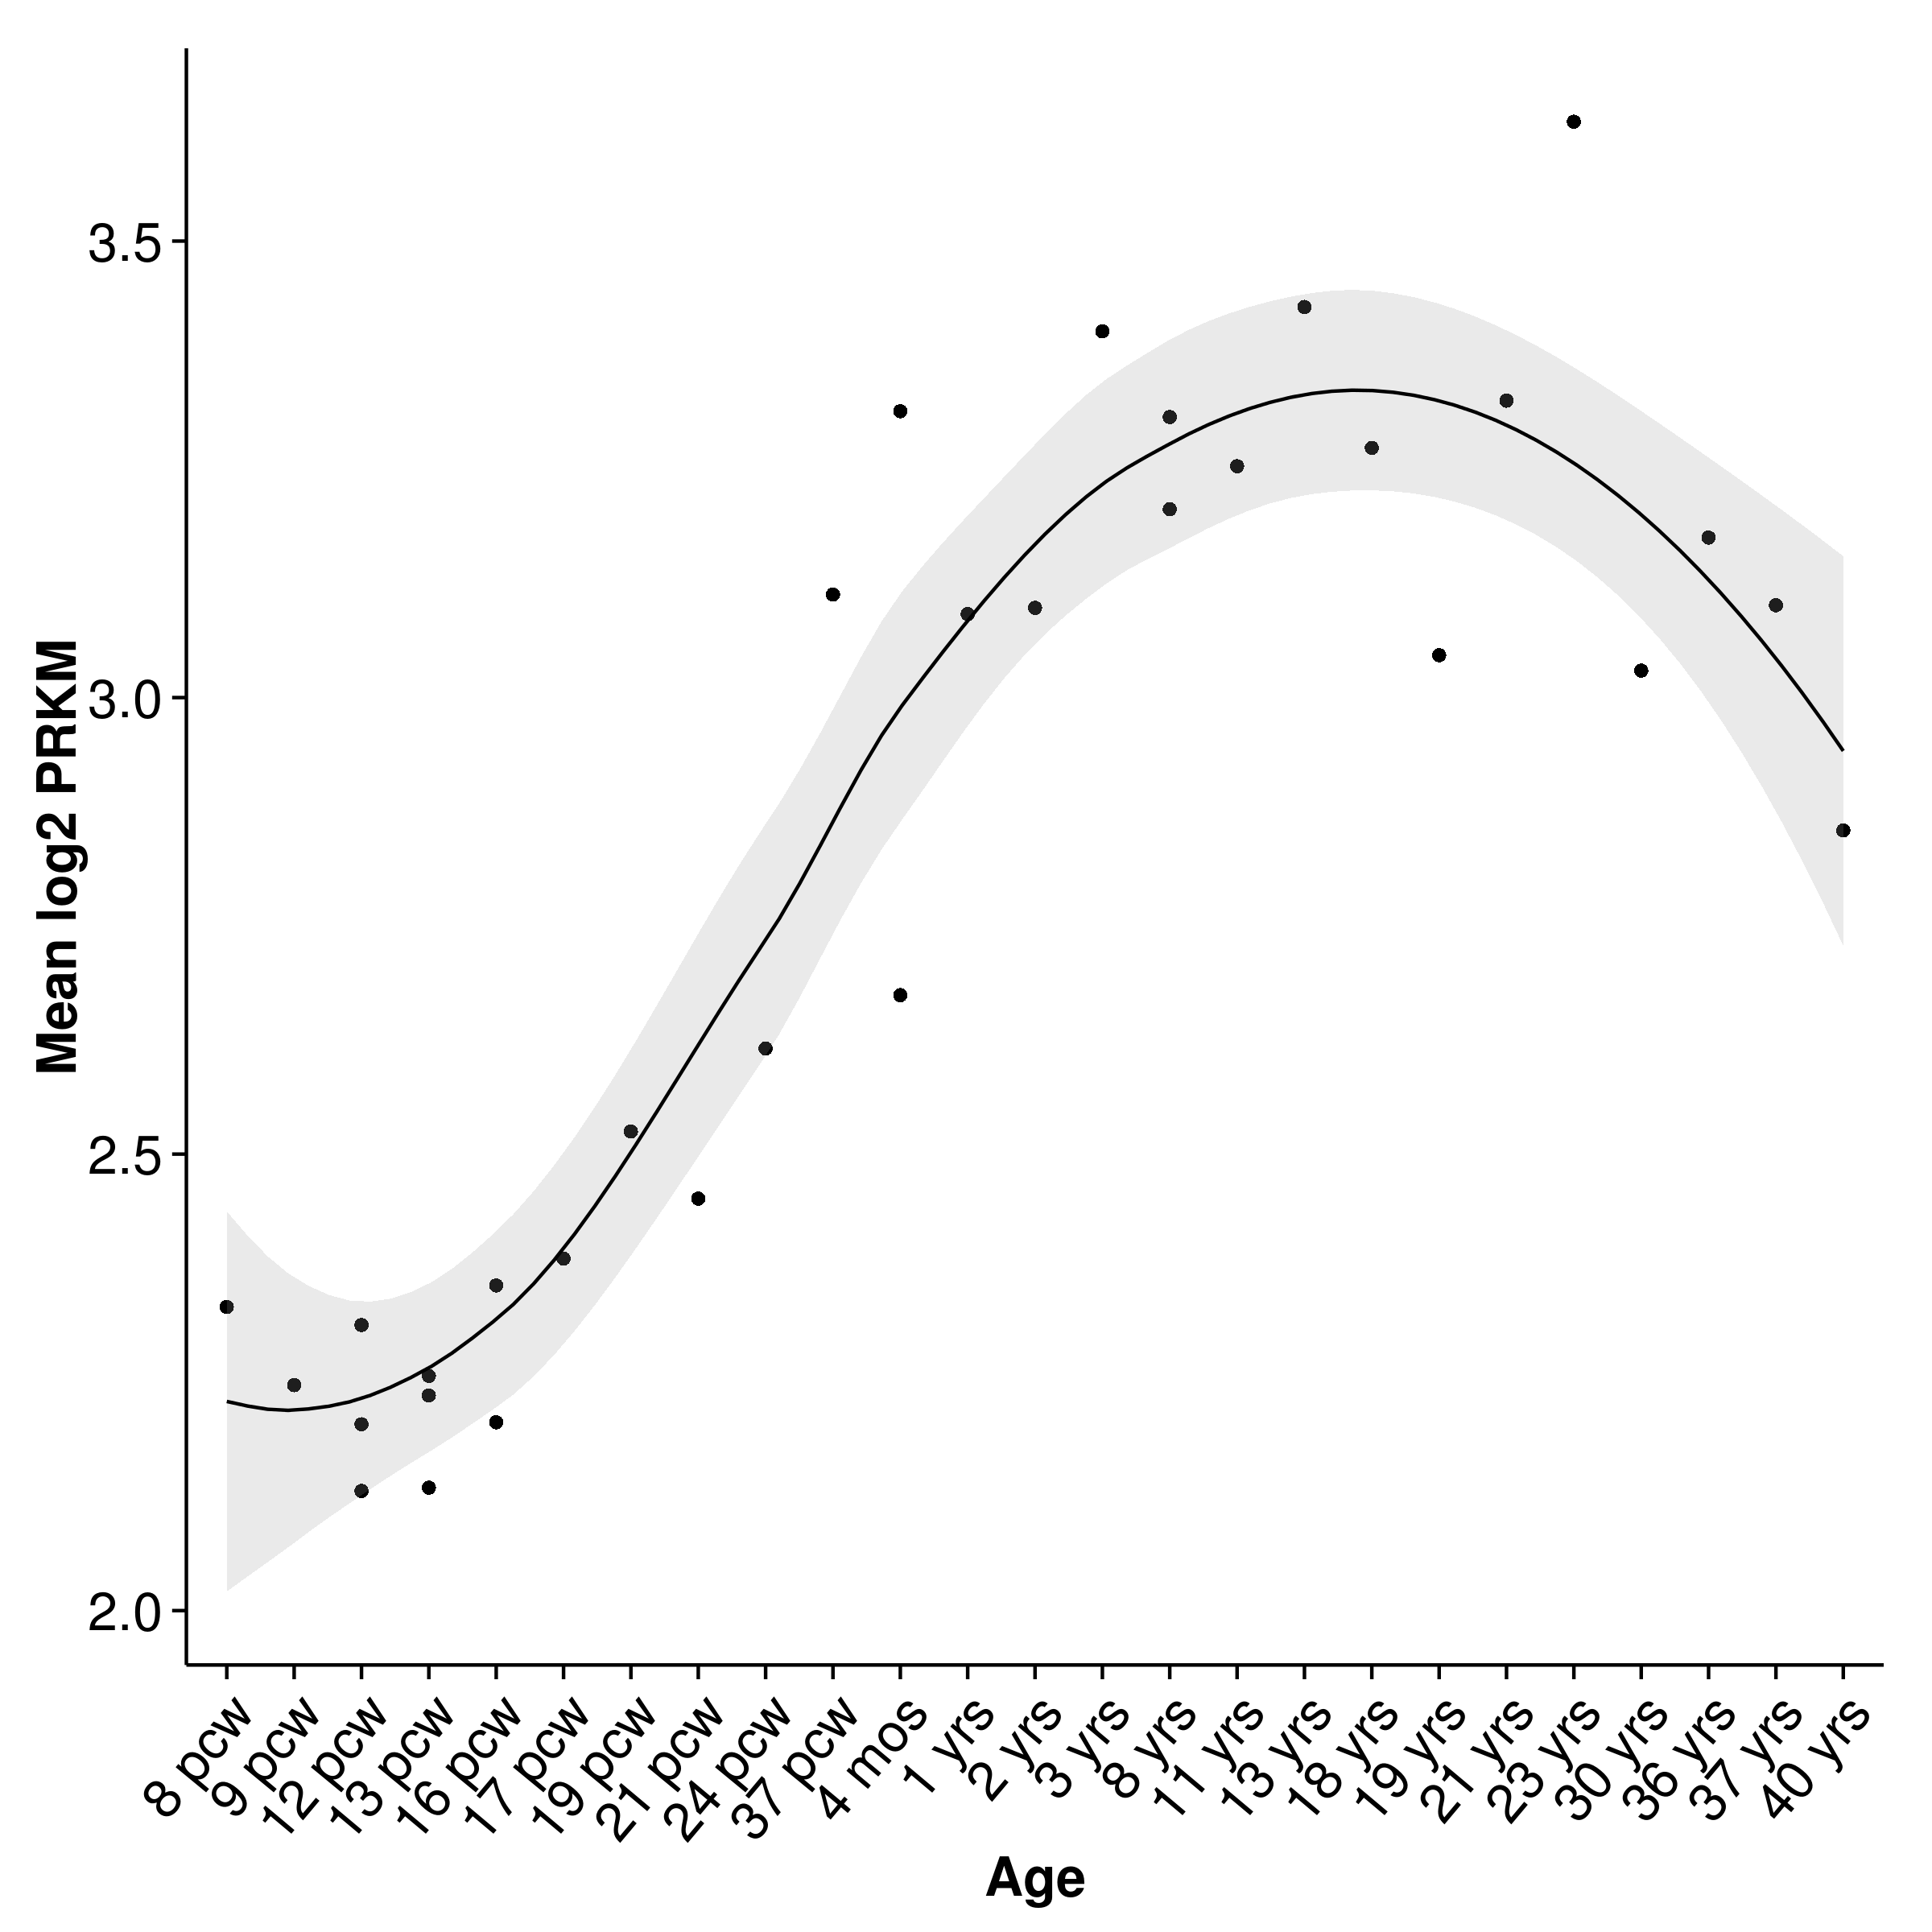
\includegraphics{figure/network/hip_network.png}}
		\label{fig:blackMod}
	}
	\subfloat[``Tan'' Network from Amygdala]{
		\scalebox{.4}{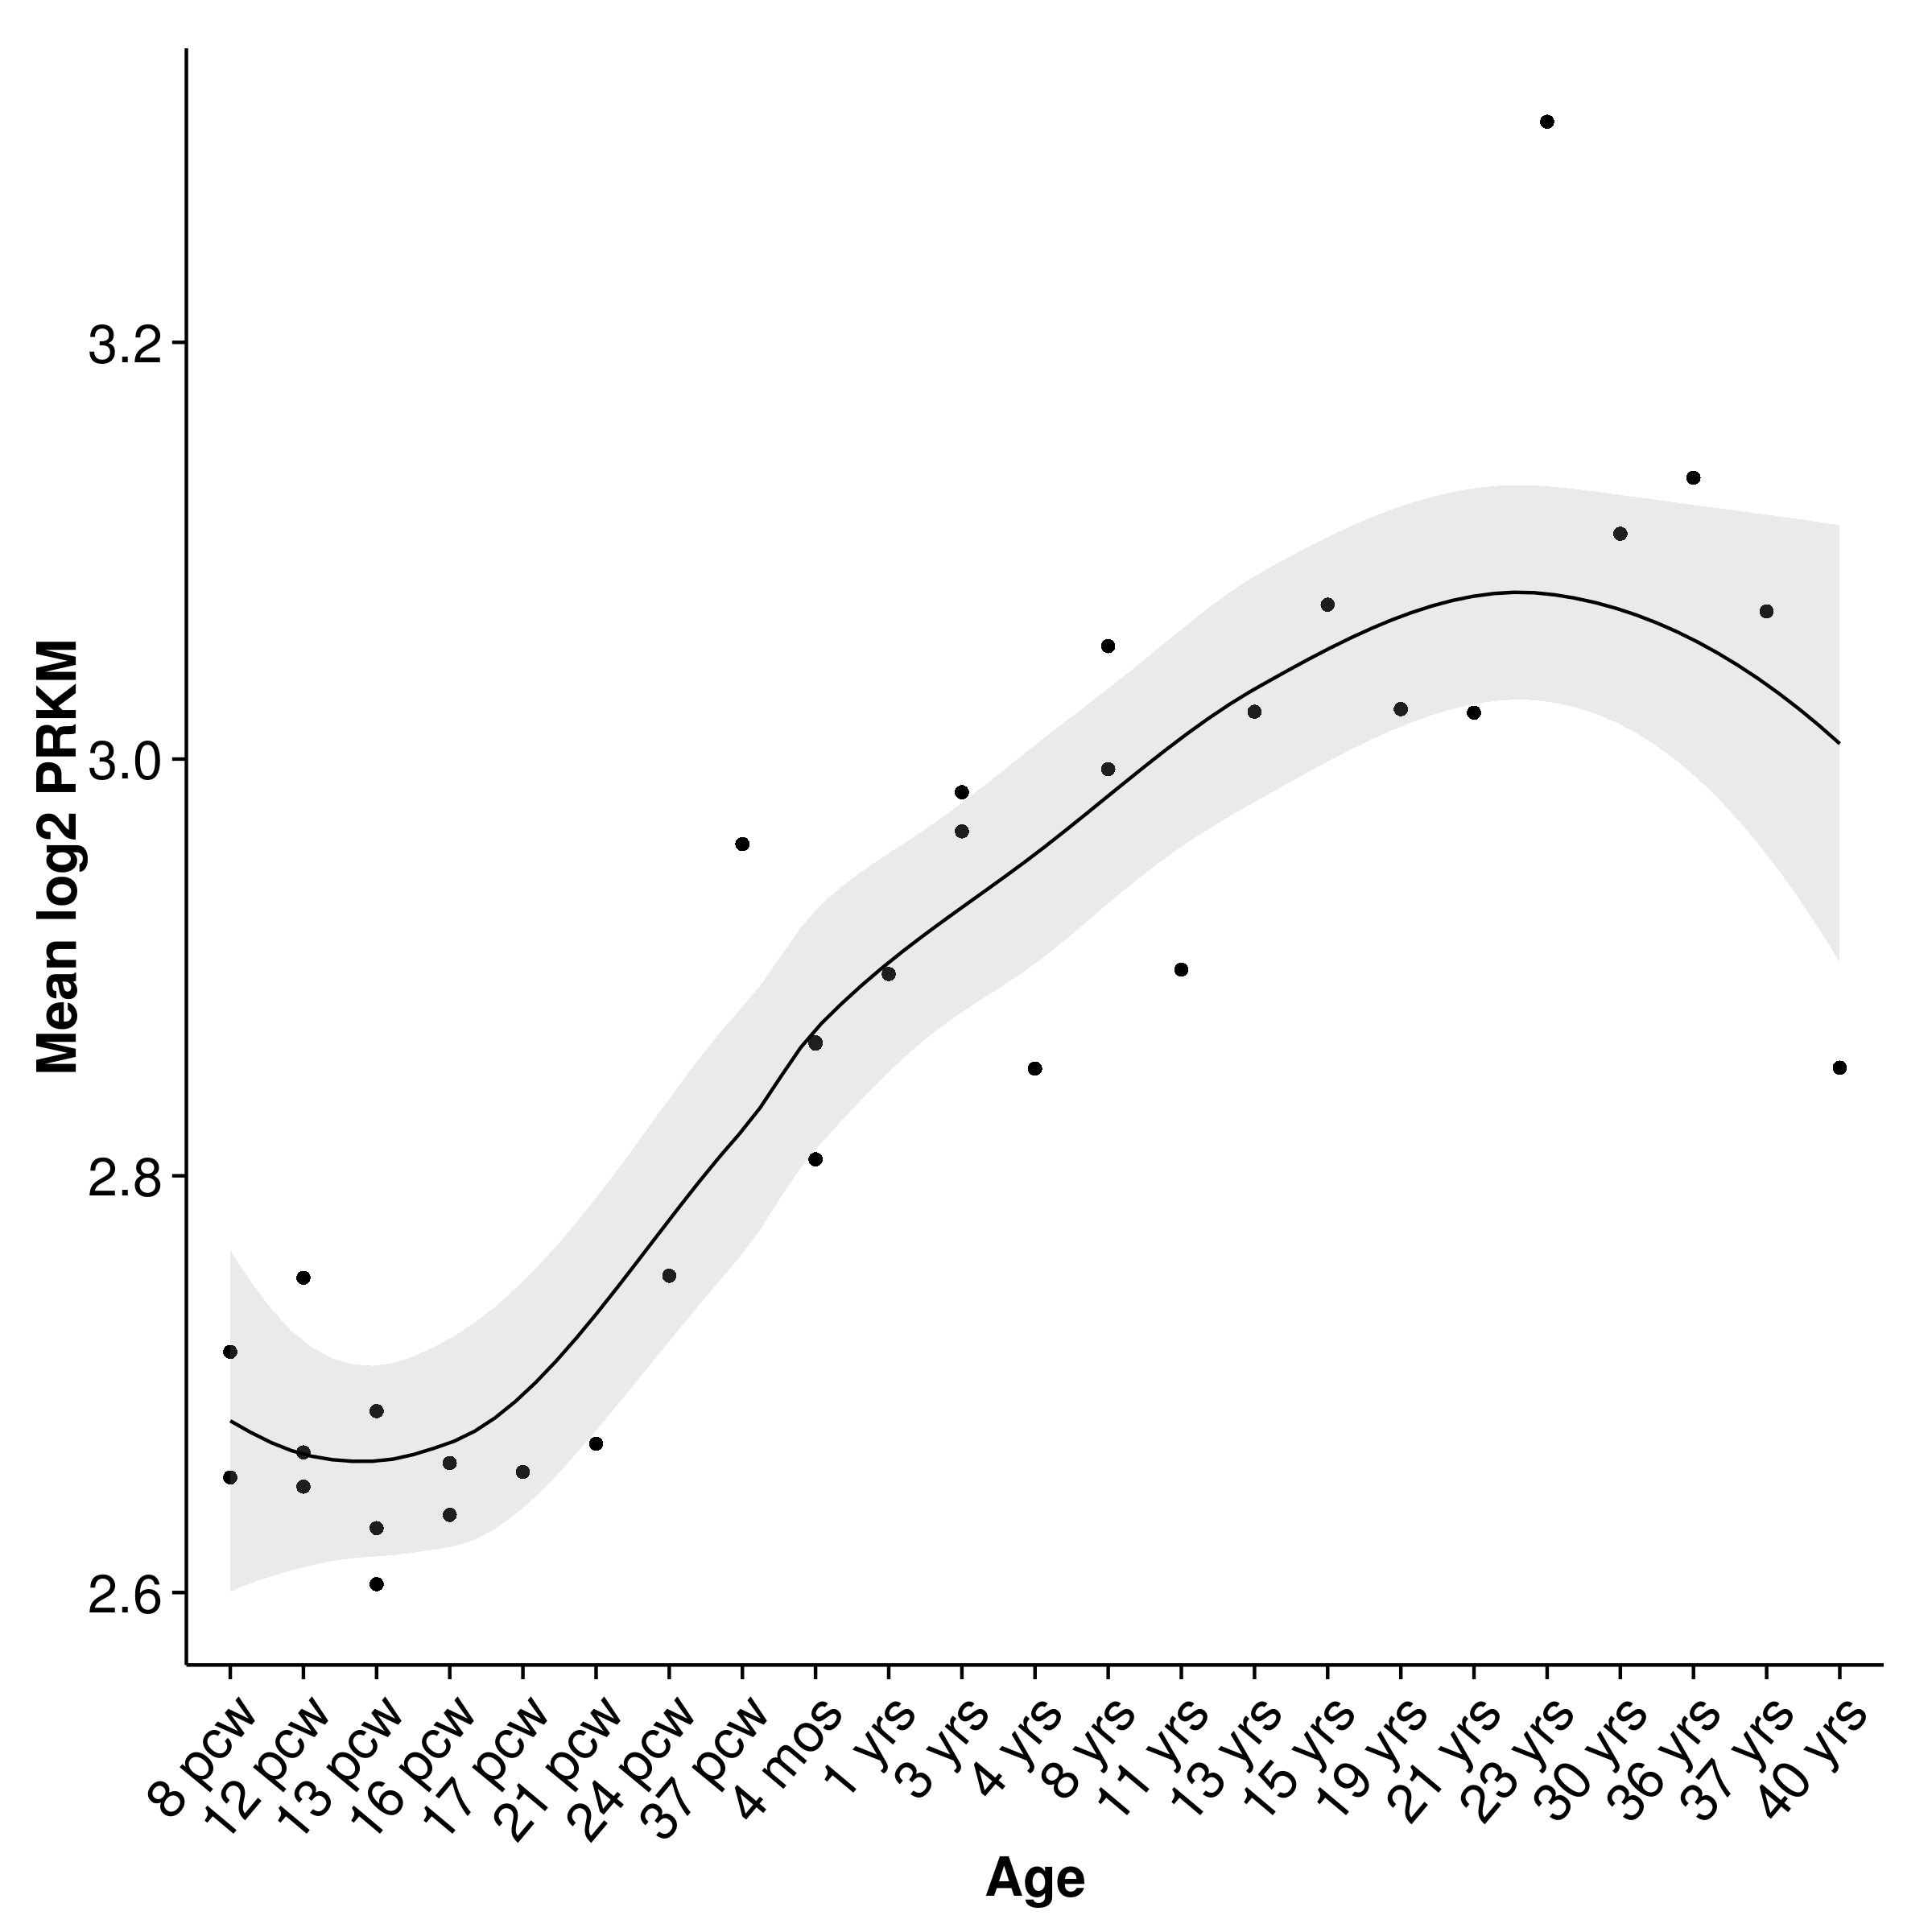
\includegraphics{figure/network/amy_tan_network}}
		\label{fig:tanMod}
	}\\
	\subfloat[``Pink'' Network from Amygdala]{
		\scalebox{.4}{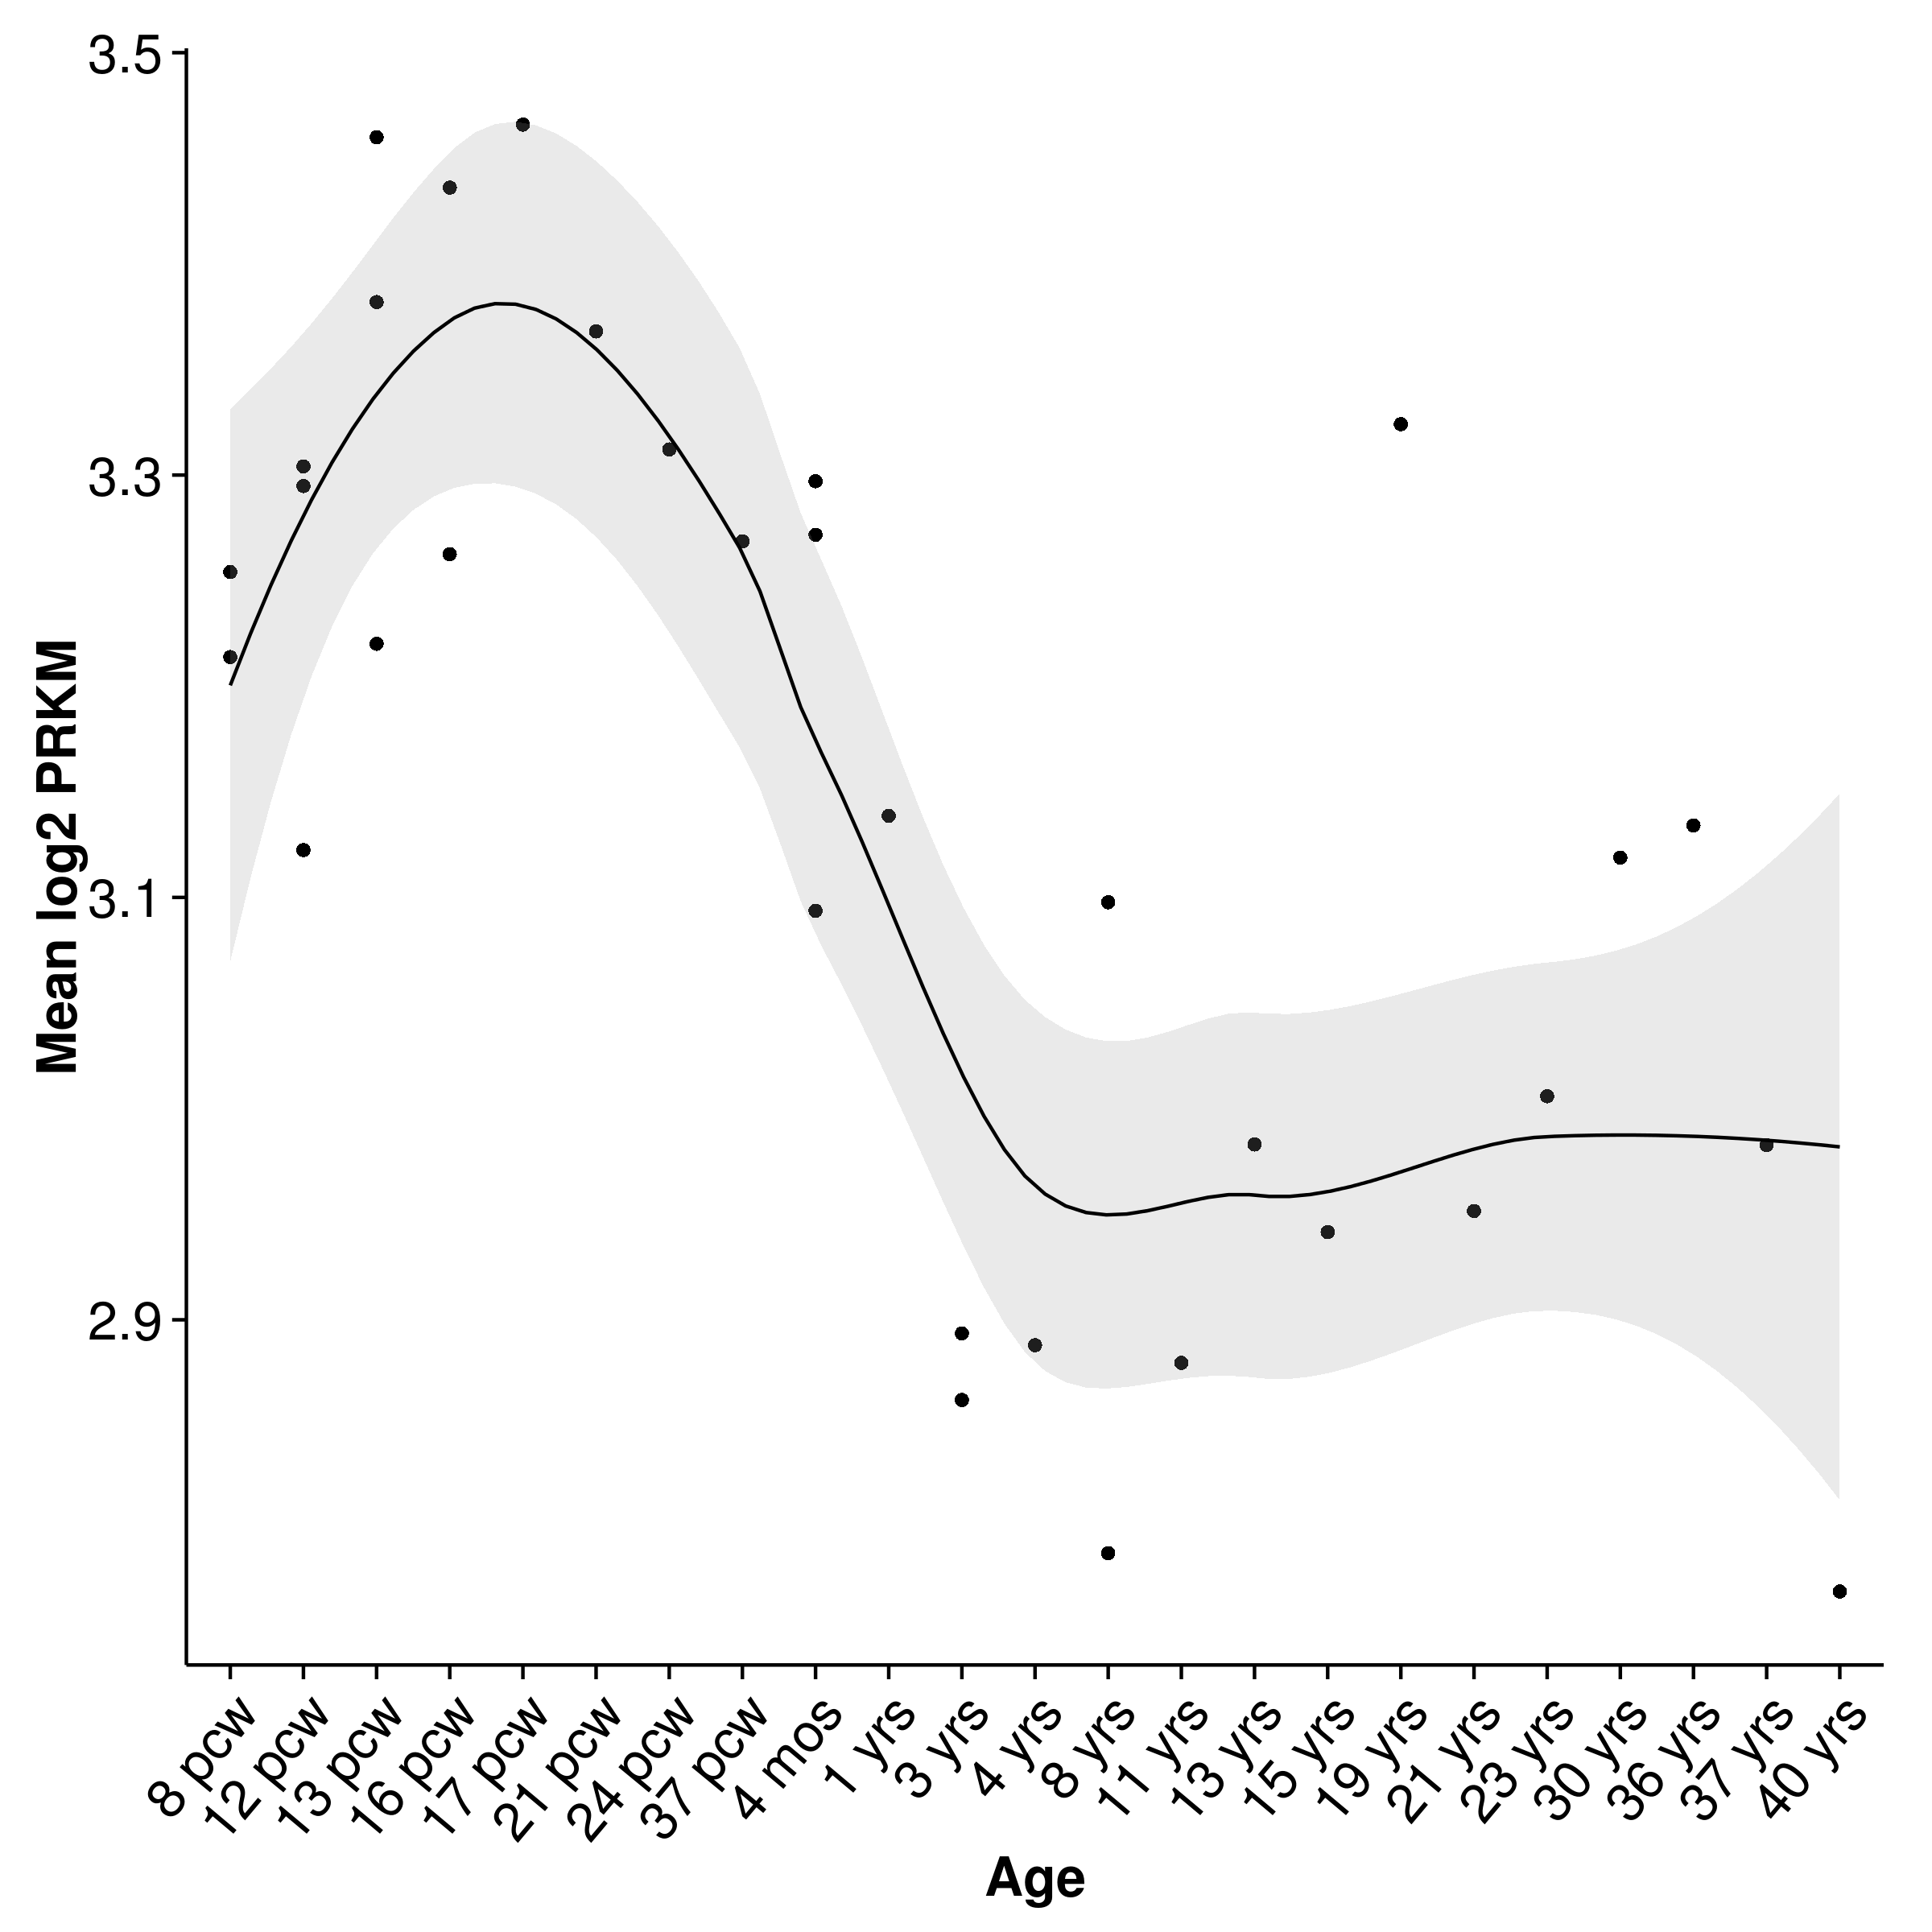
\includegraphics{figure/network/amy_pink_network}}
		\label{fig:pinkMod}
	}
	\subfloat[``Yellow'' Network from Amygdala]{
		\scalebox{.4}{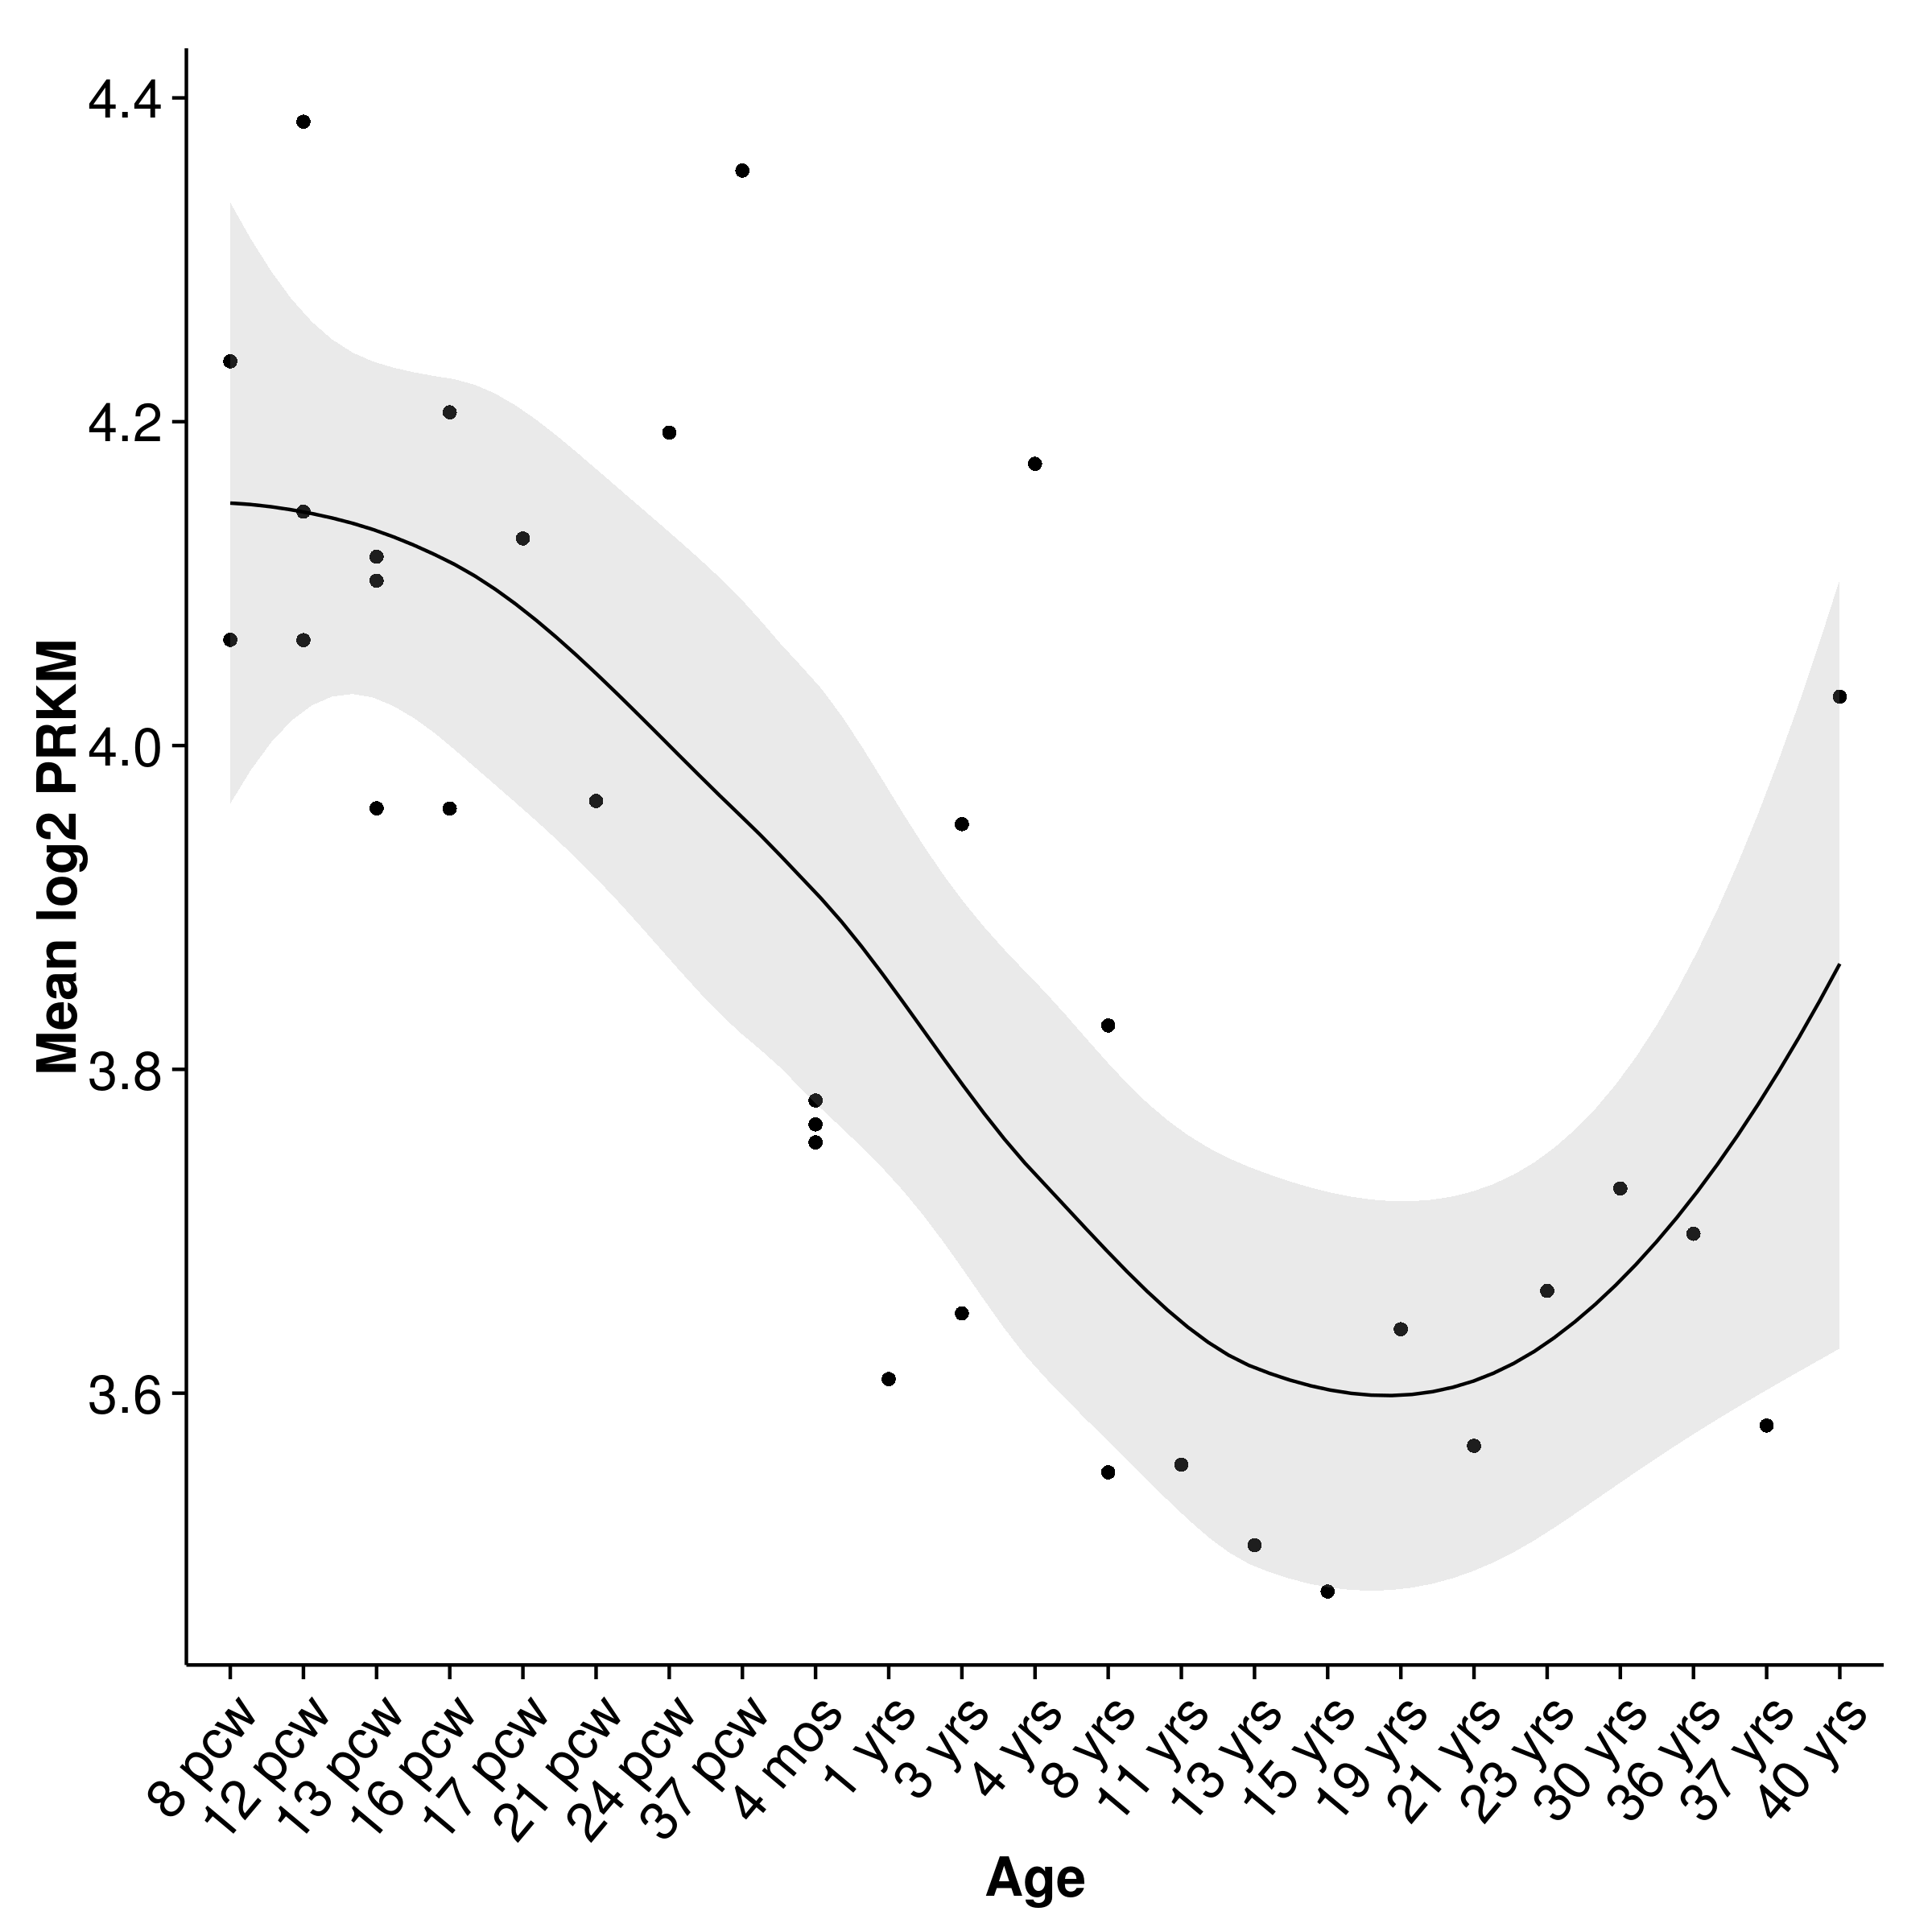
\includegraphics{figure/network/amy_yellow_network}}
		\label{fig:yellowMod}
	}
	\label{fig:allMod}
\end{figure}



\subsubsection{Functional Annotation}
Upon performing the \gls{GO} enrichment analysis, a total of 16 \gls{GO} terms were enriched in the ``black'' hippocampus network, 4 in the ``tan'' amygdala network and 45 in the ``yellow'' amygdala network. 
No \gls{GO} term was enriched in the ``pink'' amygdala network.

The enriched \gls{GO} terms of the ``yellow'' amygdala network were mainly related to translation and transcription and were not specific to brain function or development(\cref{tab:yellowGO}). 
On the contrary, the \gls{GO} terms enriched in the ``black'' hippocampus network were highly relevant to brain function and development (\cref{tab:blackGO})(e.g. ``central nervous system development'' and ``glutamate metabolic process'') and the ``tan'' amygdala network were also related to ammonium ion metabolism (\cref{tab:tanGO}) which is vita for glutamine synthesis from glutamate\citep{Liaw1995}. 

Together, it is highly likely that the ``black'' hippocampus and ``tan'' amygdala networks are related to brain development and function.

\begin{table}[h]
	\centering
	\caption[\glsentryshort{GO} enrichment results for the ``black'' network from Hippocampus]{\gls{GO} enrichment results for the ``black'' network from Hippocampus.
		Among the enriched \gls{GO} terms, it was most interesting to identify a number of brain developmental related \gls{GO} terms such as ``central nervous system development'', ``axon ensheathment in central nervous system'', ``glutamate metabolic process'' and ``positive regulation of gliogenesis''. 
		Surprisingly, \gls{GO} related to immune systems were also observed ``positive regulation of production of molecular mediator of immune response''.
	}
	\begin{tabular}{rrr}
		\toprule
		term\_ID & description & p-value \\
		\midrule
		GO:0019752 & carboxylic acid metabolic process & $4.92\times 10^{-6}$ \\
		GO:0007417 & central nervous system development & $5.94\times 10^{-5}$ \\
		GO:0002821 & positive regulation of adaptive immune response & $6.12\times 10^{-5}$ \\
		GO:0006082 & organic acid metabolic process & $1.03\times 10^{-3}$ \\
		GO:0032291 & axon ensheathment in central nervous system & $1.86\times 10^{-3}$ \\
		GO:1901565 & organonitrogen compound catabolic process & $1.99\times 10^{-3}$ \\
		GO:0006536 & glutamate metabolic process & $3.54\times 10^{-3}$ \\
		GO:0021762 & substantia nigra development & $3.73\times 10^{-3}$ \\
		GO:0044281 & small molecule metabolic process & $4.34\times 10^{-3}$ \\
		GO:0030194 & positive regulation of blood coagulation & $4.59\times 10^{-3}$ \\
		GO:0009607 & response to biotic stimulus & $6.14\times 10^{-3}$ \\
		GO:0002702 & positive regulation of production of molecular mediator of immune response & $6.21\times 10^{-3}$ \\
		GO:0034103 & regulation of tissue remodeling & $6.21\times 10^{-3}$ \\
		GO:0014015 & positive regulation of gliogenesis & $7.47\times 10^{-3}$ \\
		GO:0098542 & defense response to other organism & $7.95\times 10^{-3}$ \\
		GO:0019835 & cytolysis & $8.72\times 10^{-3}$ \\
		\bottomrule
	\end{tabular}%
	\label{tab:blackGO}%
\end{table}%
\begin{table}[h]
	\centering
	\caption[\glsentryshort{GO} enrichment results for the ``tan'' network from Amygdala]{\gls{GO} enrichment results for the ``tan'' network from Amygdala.
		Unlike the ``black'' network, only a small number of \gls{GO} terms were enriched. 
		However, these \gls{GO} terms are relatively specific to amine/ammonium ion metabolism.
		Interestingly, ammonium ion are essential to the synthesis of glutamine from glutamate, suggesting that this network might be relate to the glutamate system.
	}
	\begin{tabular}{rrr}
		\toprule
		term\_ID & description & p-value \\
		\midrule
		GO:0097164 & ammonium ion metabolic process & $1.37\times 10^{-3}$ \\
		GO:0044106 & cellular amine metabolic process & $4.2\times 10^{-3}$ \\
		GO:0009308 & amine metabolic process & $5.41\times 10^{-3}$ \\
		GO:0046519 & sphingoid metabolic process & $6.01\times 10^{-3}$ \\
		\bottomrule
	\end{tabular}%
	\label{tab:tanGO}%
\end{table}%

\subsubsection{Associate Co-expression network with \glsentryshort{pgc} schizophrenia data}
Although the co-expression network were extremely interesting for their expression pattern and functional enrichment in brain development and function related \gls{GO} terms, there were no evidence of their involvement nor importance in schizophrenia.
Therefore it is of particular interest for us to test whether if genes within these co-expression networks were associated withs schizophrenia. 

First, gene base p-value of 18,622 genes were calculated using p-values from the \gls{pgc} schizophrenia working group\citep{Ripke2014}.
Gene set enrichment analysis were then performed using \gls{MAGMA}\citep{DeLeeuw2015} to test whether if there genes within the ``black'' hippocampus and ``tan'' amygdala networks were significantly associated with schizophrenia.

Based on the self-contained gene set enrichment analysis, genes within both networks were significantly associated with schizophrenia with p-value of $1.38\times 10^{-41}$ for the ``tan'' amygdala network and $2.70\times 10{-74}$ for the ``black'' hippocampus network.
These suggest that these networks might be disrupted in schizophrenia patients.
%Network	Size	self-contained	competitive
%Amygdala        289   1.3869e-41      0.44715
%Hippocampus     458   2.6993e-74      0.20002




\subsubsection{Partitioning of Heritability}

\section{Discussion}